\documentclass[11pt]{scrreprt}
\usepackage[utf8]{inputenc}

\title{\textbf{Project 2 Report}}
\subtitle{CS325 Analysis of Algorithms, Summer 2015}
\author{\textsf{\textbf{Project Group 1}}\\
		\textsf{Tingzhi Li}\\
		\textsf{Nicholas Nelson}\\
		\textsf{Chunyang Zhang}}
		
\usepackage{graphicx}

\usepackage{listings} %插入代码
\usepackage{xcolor} %代码高亮

\lstset{numbers=left, %设置行号位置
	numberstyle=\tiny, %设置行号大小
	keywordstyle=\color{blue}, %设置关键字颜色
	commentstyle=\color[cmyk]{1,0,1,0}, %设置注释颜色
	frame=single, %设置边框格式
	escapeinside=``, %逃逸字符(1左面的键),用于显示中文
	breaklines, %自动折行
	extendedchars=false, %解决代码跨页时,章节标题,页眉等汉字不显示的问题
	xleftmargin=2em,xrightmargin=2em, aboveskip=1em, %设置边距
	tabsize=4, %设置tab空格数
	showspaces=false %不显示空格
}

%\usepackage[demo]{graphicx}
\usepackage{caption}
\usepackage[labelformat=simple]{subcaption}
\renewcommand\thesubfigure{(\alph{subfigure})} % see subcaption doc


\date{}
\begin{document}

\maketitle


\chapter{Theoretical Analysis}

\section{Dynamic Programming Table Filling Logic}

The table for the dynamic programming algorithm consists of avaiable coins as the column header and the amount of change as the row header. The minimum number of coins for that particular amount of change is filled into the cells of the table according to the algorithm. The base case of this table is $T[0]=0$, which means the first row will be filled with zeroes. For $T[1]$ we need to look up $T[1-V[i]]$ where $v[i]\leq 1$. The same logic applies to all the following cases.

For example, if our avaiable coins are [1,2,5,10], $A=5$. Then the table would look like the following:\\

\begin{tabular}{|c|c|c|c|c|}
	\hline & \multicolumn{4}{|c|}{Avaiable coins' value} \\
	\hline Change & 1  & 1, 2 & 1, 2, 5 & 1, 2, 5, 10 \\ 
	\hline 0 & 0 & 0 & 0 & 0 \\ 
	\hline 1 & 1 & 1 & 1 & 1 \\ 
	\hline 2 & 2 & 1 & 1 & 1 \\ 
	\hline 3 & 3 & 2 & 2 & 2 \\ 
	\hline 4 & 4 & 2 & 2 & 2 \\ 
	\hline 5 & 5 & 3 & 1 & 1 \\ 
	\hline 
\end{tabular}\\\\

Since the table is filled in from the base case, for each step it is possible to guarantee that the optimal number of coins needed for a particular amount of change is found based upon previously derived solutions. This allows the dynamic algorithm to arrive at the optimal solution to any target amount of change.


\section {Pseudo-Code and Theoretical Running-Time Analysis}


\subsection {Brute Force Algorithm}

\begin{lstlisting}[language=c]
function changeslow(V[n],A){
	C[n] = [0,...,0]
	for (j = 0; j < n; j++){
		if (A == V[j]){
			m = 1
			C[j] += 1
			return m, C[n]
	}
	min = A
	for (i = 1; i < A; i++){
		m1, c1[n] = changeslow(V[n], i)
		m2, c2[n] = changeslow(V[n], A - i)
		m = m1 + m2
		c[n] = c1[n] + c2[n]
		if (min > m){
			min = m
			Cmin[n] = c[n]
		}
	}
	return min, Cmin[n]
}
\end{lstlisting}

In this algorithm, the running-time complexity is given by:
\begin{eqnarray*}
T(n) 	& = & (T(1)+ T(n-1)) + (T(2) + T(n-2)) + ... + (T(n-1) + T(1)) + c\\
		& = & 2(T(1) + T(2) + T(3) + ... + T(n-1)) + c\\
T(1)	& = & c\\
T(2) 	& = & 2T(1) + c\\
T(3) 	& = & 2(1+2)T(1) + (1+2)c\\
T(4) 	& = & 2(1+2+2(1+2))T(1) + (1+2+4)c\\
	 	& = & (2+4)(1+2)T(1) + (1+2+4)c\\
T(5) 	& = & (2+4+8)(1+2)T(1) + (1+2+4+8)c\\
		& . & \\
		& . & \\
		& . & \\
T(n) 	& = & (2+4+8+16+..+2^{n-2})(1+2)T(1) + (1+2+4+8+...+2^{n-2})c\\
		& = & (2^{n-1}-2)T(1) + 2^{n-1}c\\
		& = & (2^n-2)c\\
		& = & \Theta(2^n)\\
\end{eqnarray*}

Note that the $n$ is the target change amount; not the index number of the list.

\subsection{Greedy Algorithm}

\begin{lstlisting}[language=c]
function changegreedy(V[n],A) {
	reverse(V[n])
	c[n] = [0,...,0]
	for (i = 0; i < n; i++){
		temp = A - V[i]
		while (temp >= 0){
		    A = temp
		    c[i] += 1
		    m += 1
		    temp = A - V[i]
		}
	}
	return c, m
}
\end{lstlisting}

In this algorithm, the running-time complexity is:
\begin{eqnarray*}
T(n) = \Theta(n)
\end{eqnarray*}
 where $n$ is the target change amount.
\subsection{Dynamic Programming}

\begin{lstlisting}[language=c]
function changedp(V[n], A){
	c[A][n] = [[0,...,0],...,[0,...,0]]
	T[A] = [0,...,0]
	temp[n] = [0,...,0]
	for (i = 1; i <= A; i++){
		for (j = 0; j < n; j++){
			k = j - V[j]
			if (k >= 0){
				temp[j] = T[k] + 1
		T[i] = min(temp[j])				\\The index of the minimum value of array temp is j.
		c[i][j] = c[k][j] + 1
	}
	return c[A], T[A]
}
\end{lstlisting}

In this algorithm, the running-time complexity is:
\begin{eqnarray*}
T(n) = \Theta(Cn)
\end{eqnarray*}

where $C$ is the number of different kinds of coins and $n$ is the target change amount.


\section{Proof for Dynamic Programming}


The pseudo-code for Dynamic Programming is shown above in Section 1.2.3.\\

As proved before, the running time for this method is
\begin{eqnarray*}
T(n)  =  \Theta(Cn)
\end{eqnarray*}

where $C$ is the number of different kinds of coins and $n$ is the target change amount.\\

In this programming method,\\

\emph{Precondition:}

1. Array $V[n]$ is sorted, of which the minimum value is always 1.
 
2. Number $v$ that needed to be turned into change is a positive integer which is greater than 0.\\

\emph{Postcondition:}

1. The minimum number of coins cost is found.

2. The number of each coin cost is found.\\

\ \ For
\begin{eqnarray*}
T[v] = min\{T[v - V[i]] + 1\},\ T[0] = 0
\end{eqnarray*}

\emph{Precondition:}

$v - V[i]$ is greater than or equal to 0.\\

\emph{Postcondition:}

The minimum of $T[v - V[i]] + 1$ is found.\\

\emph{Base Case:}

$T[0] = 0$\\

\emph{Inductive Hypothesis:}

Assume $T[v - V[i]]$ is the minimum of $T[(v - V[i]) - V[j]]$.\\

\emph{Inductive Step:}

Show that $T[n]$ is the minimum.

-\ First, $T[0]$ is 0, which is already the minimum.

-\ Second, $T[1]$ is calculated by using $T[0]$, which is also the minimum.

-\ Third, $T[k]$ is calculated by using $T[k - V[i]]$, where

\ \ 1. $T[k - V[i]]$ is now fulfill the precondition of $T[v]$.

\ \ 2. The postcondition of $T[v]$ guarantees that $T[k]$ is minimum.\\

\emph{Termination:}

At termination, $T[v] = T [v - V[i]]$. Set $T[k] = T[v - V[i]]$, Then $T[k] = T[k - V[i]]$. By the loop to choose the minimum, each $k$ will terminate at several $k - V[i]$ and choose the smallest value of $T[k] + 1$, where each $T[k - V[i]]$ is already at its minimum value because all of the $T[k]$ will depend all the way back on to $T[0]$, which is 0. This loop will guarantee the $T[v]$ gets its minimum.


\chapter{Experimental Analysis}

\section{Situation 1}
\label{sec:sit1}

Figure~\ref{fig:p4} is the graph of the number of coins required (y-axis) to make change for $A$ (x-axis) for the Greedy and Dynamic Programming algorithms where $V = [1, 5, 10, 25, 50]$ and $A$ is values in $[2010, 2015, 2020, ..., 2200]$  (per problem 4 of the project instructions). Although the Greedy algorithm is not guaranteed to derive the minimum number of coins for a any given $A$, the specific set of coins ($V$) in this case allows it to be correct for all values of $A$.

\begin{figure}[!htbp]
\centering
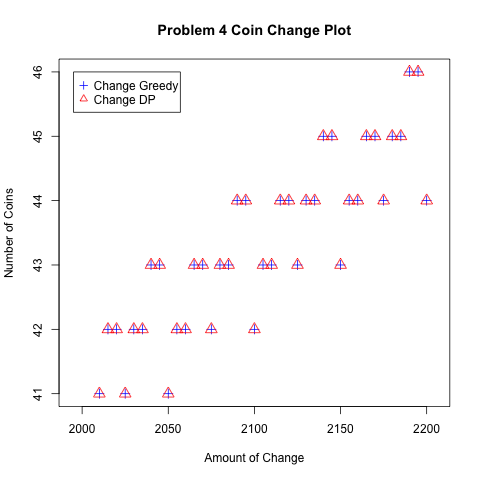
\includegraphics[width=8cm]{situation1.png}
\caption{Number of coins vs. target change values for Greedy \& Dynamic Programming algorithms (problem 4, set V)}
\label{fig:p4}
\end{figure}

\section{Situation 2}
\label{sec:sit2}

Figure~\ref{fig:p5} is the graphs of the number of coins required (y-axis) to make change for $A$ (x-axis) for the Greedy and Dynamic Programming algorithms where $V_1 = [1, 2, 6, 12, 24, 48, 60]$, $V_2 = [1, 6, 13, 37, 150]$, and $A$ is values in $[2000, 2001, 2002, ..., 2200]$ (per problem 5 of the project instructions). Since the Greedy algorithm is not guaranteed to derive the minimum number of coins required for all values of $A$, the results show the number of coins differing between the two algorithms throughout the range of values for $A$.

\begin{figure}[!htbp]
	\captionsetup{justification=centering,singlelinecheck=off}
	\captionsetup[subfigure]{singlelinecheck=on}
	%
	\captionbox{Number of coins vs. target change values for Greedy \& Dynamic Programming algorithms (problem 5, set V\textsubscript{1}; problem 5, set V\textsubscript{2}) 
	\label{fig:p5}}[1.0\textwidth]
	{%
		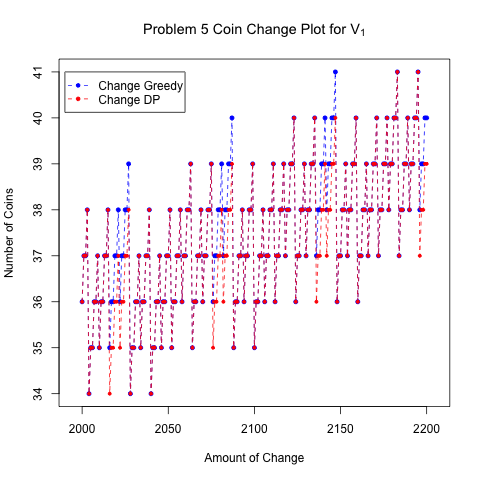
\includegraphics[width=0.50\textwidth]{situation2_1.png}%
		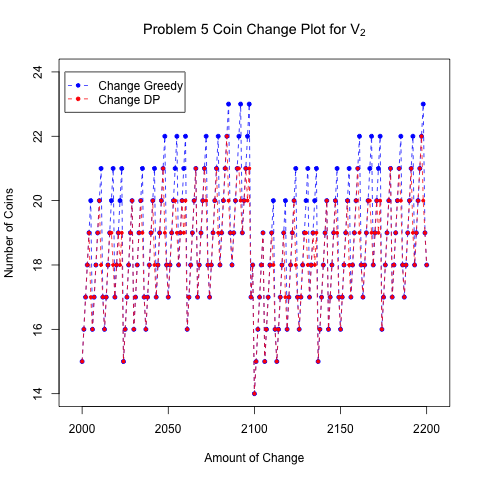
\includegraphics[width=0.50\textwidth]{situation2_2.png}
	}%
\end{figure}

\newpage
\section{Situation 3}
\label{sec:sit3}

Figure~\ref{fig:p6} is the graph of the number of coins required (y-axis) to make change for $A$ (x-axis) for the Greedy and Dynamic Programming algorithms where $V = [1, 2, 4, 6, 8, 10, 12, ..., 30]$ and $A$ is values in $[2000, 2001, 2002, ..., 2200]$ (per problem 6 of the project instructions). Although the Greedy algorithm is not guaranteed to derive the minimum number of coins for any given $A$, the specific set of coins ($V$) in this case allows it to be correct for all values of $A$.

\begin{figure}[!h]
\centering
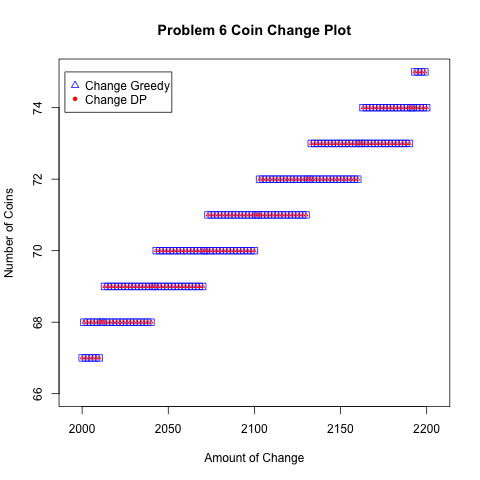
\includegraphics[width=8cm]{situation3.png}
\caption{Number of coins vs. target change values for Greedy \& Dynamic Programming algorithms (problem 6, set V)}
\label{fig:p6}
\end{figure}

\section{Running Time Comparison}
\label{sec:timings}

Figure~\ref{fig:p4_time}, \ref{fig:p5_v1_time}, \ref{fig:p5_v2_time}, and \ref{fig:p6_time} all present the individual timing graphs for both the Greedy Algorithm and Dynamic Programming, with their respective scales for time (ms), and a combined graph for comparision between both algorithms.

\section{Exploring Relationship Between Running Time and Number of Denominations}

Based upon the data presented in section~\ref{sec:sit1}, section~\ref{sec:sit2}, section~\ref{sec:sit3}, and section~\ref{sec:timings}, we can experimentally deduce that the number of denominations ($n$) has a positive (increasing time) effect for determining the minimum number of coins to make change.

The Greedy Algorithm must potentially search through all possible coins ($n$) in determining a solution, so the size of $n$ has an effect on the run-time of this algorithm. This effect is minimal since the algorithm must search through the set of coins at most once.

The Dynamic Programming method must calculate the minimum number of coins for each sub-problem ($i$) by comparing against all possible coins ($n = |V|$) where $V_i <= v$ and $v$ is the target value at that step. Since the number of sub-problems is determined by the number of coins (of value less than the target), $n$ directly factors into the overall run-time of this algorithm.

\section{Special Coins Value Case}

\ \ \ If the coins have values that are powers of $p$, namely $V = [p^0 , p^1 , p^2 , ... , p^n]$, then the dynamic programming and greedy approaches would generate the same result as each other.\\

The reason is that every larger coin is a multiple of its lower level coin, so that when the number of lower level coin satisfy a number of p, it will count to the larger one. For instance, consider $p^2 = p*p$. If there are $(p-1)*p$ amount of money that needed to be changed, the result will be $p-1$ $p^1$ coins, which is the minimum cost. But when there are $p^2$ amount of money, the result will be 1 of $p^2$ coin. The same idea satisfy all of the larger coins. Therefore, if we use Dynamic Programming Method, it will choose the minimum number when the change approaches $p^i$. If we use Greedy Algorithm, we will consider the largest power of p, and then calculate the lower level power of p and so on. In this case, although the order of this algorithm is reversed from Dynamic Programming Method but the result would be the same because they all depend on the power of p. In this case, the result of coins cost will be the same.

However, if we consider the running-time complexity, the Greedy Algorithm would be faster than Dynamic Programming Method. As we proved before, the running time for these two approaches are:
\begin{eqnarray*}
\mbox{Dynamic Programming}&:& \Theta(Cn)\\
\mbox{Greedy Algorithm}&:& \Theta(n)\\
\end{eqnarray*}

From this we can see that the Greedy Algorithm only depends on the amount of money needed to be changed, yet the Dynamic Programming depends on not only the amount, but also how many kinds of coins there are. Accordingly, the Greedy Algorithm would be faster in contrast to Dynamic Programming, especially when the amount of money is very large.

\begin{figure}[!htbp]
	\captionsetup{justification=centering,singlelinecheck=off}
	\captionsetup[subfigure]{singlelinecheck=on}
	%
	\captionbox{Time to completion (ms) vs. target change values for Greedy \& Dynamic Programming algorithms (problem 4, set V) 
	\label{fig:p4_time}}[1.0\textwidth]
	{%
		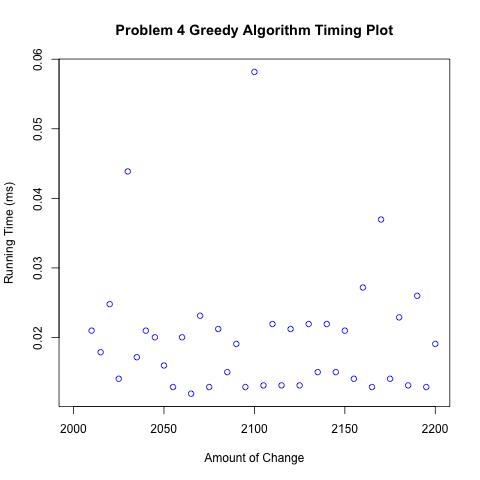
\includegraphics[width=0.50\textwidth]{time1greedy.png}%
		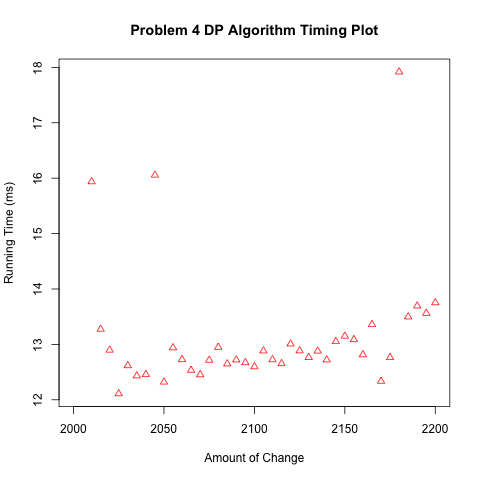
\includegraphics[width=0.50\textwidth]{time1dp.png}
		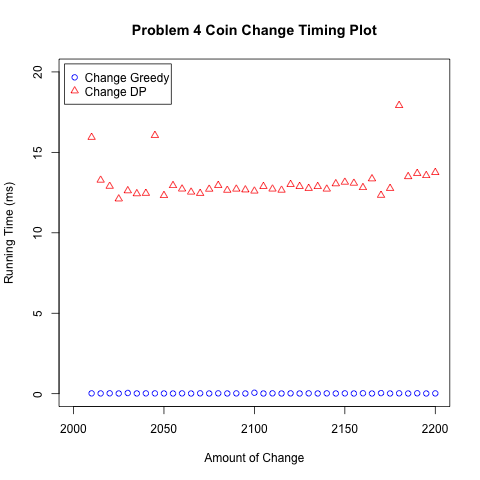
\includegraphics[width=1\textwidth]{time1.png}%
	}%
\end{figure}

\begin{figure}[!htbp]
	\captionsetup{justification=centering,singlelinecheck=off}
	\captionsetup[subfigure]{singlelinecheck=on}
	%
	\captionbox{Time to completion (ms) vs. target change values for Greedy \& Dynamic Programming algorithms (problem 5, set V\textsubscript{1}) 
	\label{fig:p5_v1_time}}[1.0\textwidth]
	{%
		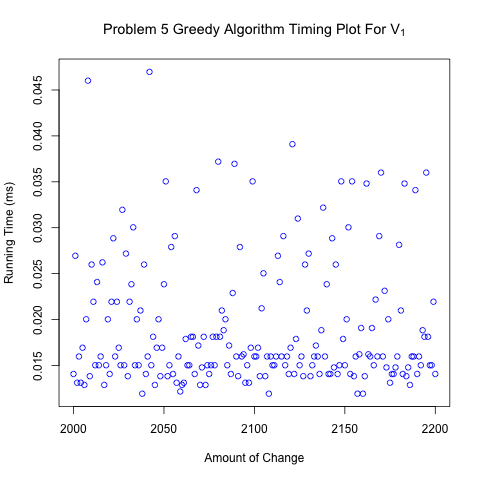
\includegraphics[width=0.50\textwidth]{time2_1greedy.png}%
		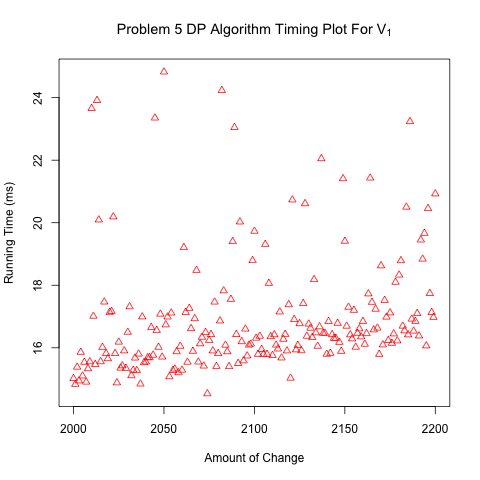
\includegraphics[width=0.50\textwidth]{time2_1dp.png}
		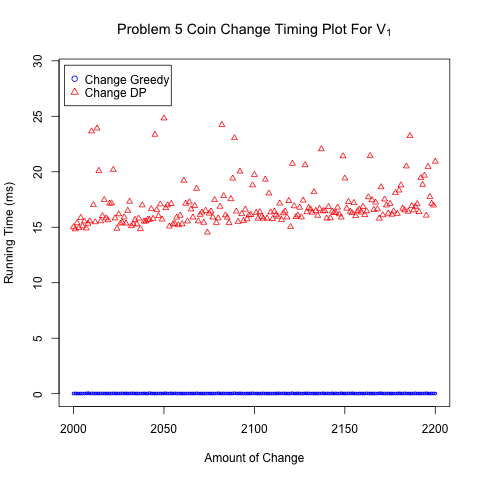
\includegraphics[width=1\textwidth]{time2_1.png}%
	}%
\end{figure}

\begin{figure}[!htbp]
	\captionsetup{justification=centering,singlelinecheck=off}
	\captionsetup[subfigure]{singlelinecheck=on}
	%
	\captionbox{Time to completion (ms) vs. target change values for Greedy \& Dynamic Programming algorithms (problem 5, set V\textsubscript{2}) 
	\label{fig:p5_v2_time}}[1.0\textwidth]
	{%
		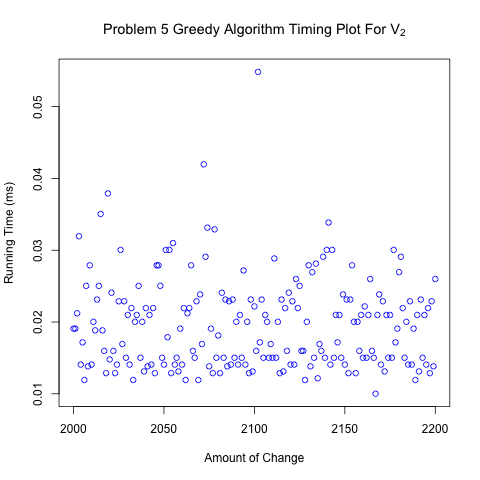
\includegraphics[width=0.50\textwidth]{time2_2greedy.png}%
		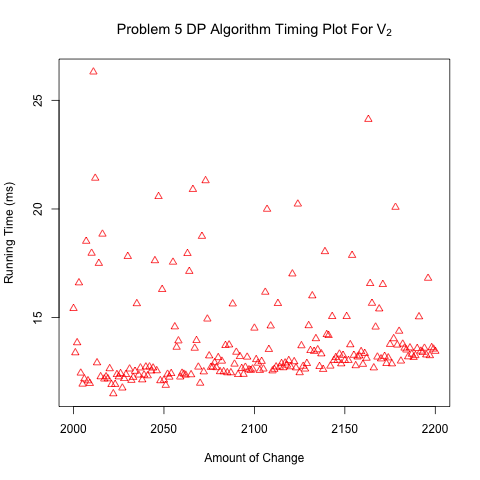
\includegraphics[width=0.50\textwidth]{time2_2dp.png}
		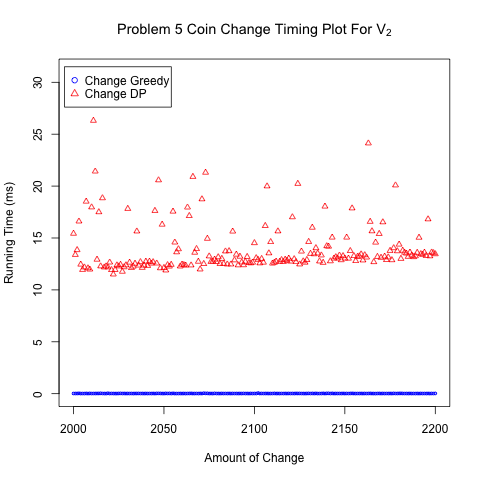
\includegraphics[width=1\textwidth]{time2_2.png}%
	}%
\end{figure}

\begin{figure}[!htbp]
	\captionsetup{justification=centering,singlelinecheck=off}
	\captionsetup[subfigure]{singlelinecheck=on}
	%
	\captionbox{Time to completion (ms) vs. target change values for Greedy \& Dynamic Programming algorithms (problem 6, set V) 
	\label{fig:p6_time}}[1.0\textwidth]
	{%
		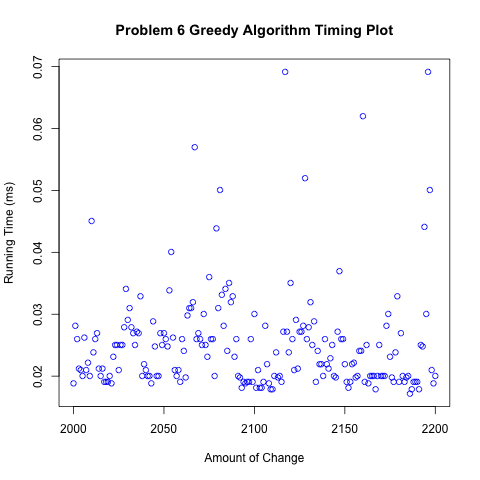
\includegraphics[width=0.50\textwidth]{time3greedy.png}%
		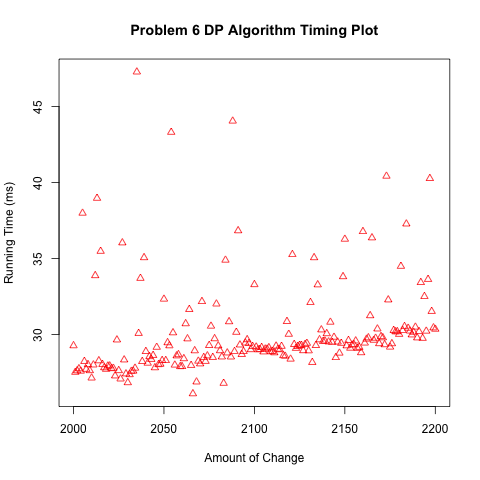
\includegraphics[width=0.50\textwidth]{time3dp.png}
		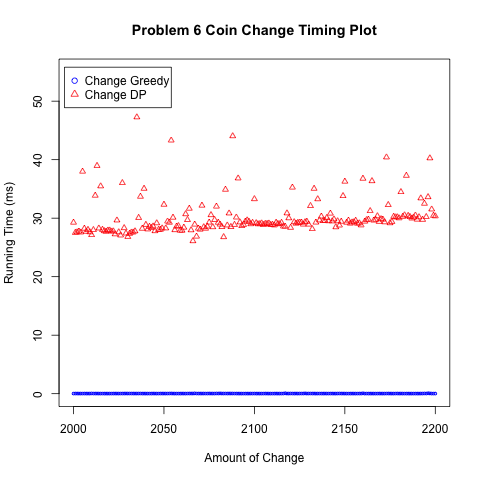
\includegraphics[width=1\textwidth]{time3.png}%
	}%
\end{figure}


\end{document} 
